%!TEX root = ../thesis_a4.tex
\chapter{Evaluation}
\label{chap:evaluation}

\section{Introduction}

One of the primary difficulties faced with designing instruments for creative and compositional tasks remains the elaboration of an appropriate evaluation methodology. Indeed, this is a trending challenge facing many researchers \citep{Barbosa2015}, and numerous papers address this directly with various proposals for methodological frameworks, some drawing from the related field of \acrshort{hci} \citep{Hsu2009, Kiefer2008a, Hiraga2004}. More generally the evaluation of computer composition systems has also been the subject of much discussion in the literature. As we alluded to in \chapref{chap:symbolic} a frequent benchmark for evaluating algorithmic music systems is a type of Turing test where the success criterion is determined by the inability of a human listener to discern between human and computer-generated music. As \citep{Abdulla2002} notes however, these kind of tests can be problematic for two reasons. Firstly, it makes the assumption that the music generated by the algorithm is intended to sound like music produced by humans, rather than something to be treated differently. Secondly it ignores other facets of the system that imperatively need evaluation, such as the interface and the experience. \cite{Pachet2015} also finds issue with simplistic Turing test approaches to music evaluation. He repeats, for instance, the view that unlike the traditional Turing test which evaluated the ability to synthesis believable natural language, no such “common-sense” knowledge exists for aspects of music.

As we were researching many of the existing works in \tabref{tab:concat_system_summary} we were struck by the absence of discussion regarding evaluation in most of the accompanying articles. Some of the articles provided descriptions of use cases \citep{Cardle2003} or at least provided links to audio examples \citep{Sturm2004}. Notably, many of the articles \citep{Simon2005}, \citep{Hackbarth2010} consistently made references to the role of “user”, but only one of those actually conducted a user experiment \citep{Aucouturier2005}. By no means is this intended to criticise the excellent work presented by these authors. Rather it is intended to highlight that although evaluation is not always an essential part of such experiments - especially in "one-off" designs for single users such as the author as composer - it is an underexplored aspect that could benefit from some contribution.

We can identify two key characteristics of our research that can inform what kind of evaluation can be carried out. Firstly it’s a retrieval system, and can be analysed to determine its ability to retrieve relevant items correctly. Secondly it is a system that involves users, or more precisely musical users. How do we evaluate this crucial facet?

Coleman has identified and addressed the lack of subjective evaluation factors in concatenative synthesis \citep{Coleman2015}. In his doctoral thesis he devotes a chapter to a listening survey conducted to determine the quality of a number of different algorithmic components of the system under consideration. He asks the listeners to consider how well the harmony and timbre of the concatenated sequences are retained. In \chapref{chap:symbolic} we conducted a similar-style listening survey to determine the ability of a genetic algorithm to create symbolic rhythmic patterns that also mimic a target input pattern. Evaluation strategies need to be tailored specifically for systems, but if the system is intended to retrieve items according to some similarity metric, and the material is musical, then a listening survey should be critical. Furthermore, and echoing Coleman's work, we would emphasise that whatever the application of a concatenative system, the evaluation of the timbral quality is essential.

We conducted extensive evaluation of our own system, both quantitatively and qualitatively. In the quantitative portion, we set out to investigate two key aspects. First, if we consider the system as a retrieval task that aims to return similar items, how accurate and predictable is the algorithm and its associated distance metric? Second, how does this objective retrieval accuracy correspond to the perceptual response of the human listener to the retrieved items? Also, rather than fit the subjective factor into some sort of haphazard Turing test box, can we determine simply if the listener likes what comes out? 

The qualitative evaluation consisted of interactive, informal interviews with intended users — mostly active music producers but also music researchers and students as they used the software. We gathered their responses and impressions and grouped them according to thematic analysis techniques. As alluded to in the introduction, both the quantitative evaluation and the qualitative evaluation have been previously reported in separate publications, but we include summaries of each here for reference.

%In light of these elements we also devised a quantitative listening survey to examine musical output of the system not only in terms of its facility in matching the target content perceptually but also in producing musically pleasing and meaningful content.

\section{System Evaluation}

We describe here the qualitative portion of the evaluation, first by introducing the experimental setup, then presenting and comparing the results of the algorithm’s retrieval accuracy with the listener survey.

\subsection{Evaluation and Experimental Design}
\label{sec:break_evaluation}

Given the rhythmic characteristics of the system we formulated an experiment that evaluated its ability to generate new loops based on acoustic drum sounds. We created a small dataset (Appendix \ref{app:resources}) of 10 breakbeats ranging from 75 BPM to 142BPM and truncated them to single bar loops. As we introduced in \chapref{chap:dancemusic} breakbeats are short drum solo sections from funk music records in the 1970s and exploited frequently as sample sources for hip-hop and electronic music. \chapref{chap:sota} also showed that computational use of breakbeats has been of interest to the scientific community, as evident in work by \cite{Ravelli2007}, \cite{Hockman2015} and \cite{Collins2006}.

Each of these loops was then used as a seed loop for the system with the sound palette derived from the remaining 9 breakbeats. Four variations were then generated with 4 different distances to the target.  These distances correspond to indices into the similarity matrix we alluded to in Section 2, which we normalise by dividing the index by the size of the table. The normalised distances then chosen were at 0.0 (the closest to the target), 1.0 (the furthest from the target) and two random distances in ranges 0.0 - 0.5 and 0.5 - 1.0.

Repeating this procedure 10 times for each target loop in the collection for each of the distance categories, we produced a total of 40 generated files to be compared with the target loop. Each step in the loop was labelled in terms of its drum content, for example the first step might have a kick and a hi-hat. Each segmented onset (a total of 126 audio samples)  in the palette was similarly labelled with its corresponding drum sounds producing a total of 169 labelled sounds. The labellings we used were K = Kick, S = Snare, HH = Hi-hat, C = Cymbal and finally X when the content wasn’t clear. \figref{fig:distrib1} shows the distribution of onsets by type in the full corpus of segmented units. Another useful statistic is highlighted in Figure \figref{fig:distrib2}, which plots the distribution of onsets for each step in the 16 step sequence for the predominant kick, snare and hi-hat for the 10 target loops. Natural trends are evident in these graphs, namely the concentration of the kick on the 1st beat, snares on the 2nd and 4th beat and hi-hats on off beats.

\begin{figure}
\centering
\begin{subfigure}[b]{0.75\textwidth}
   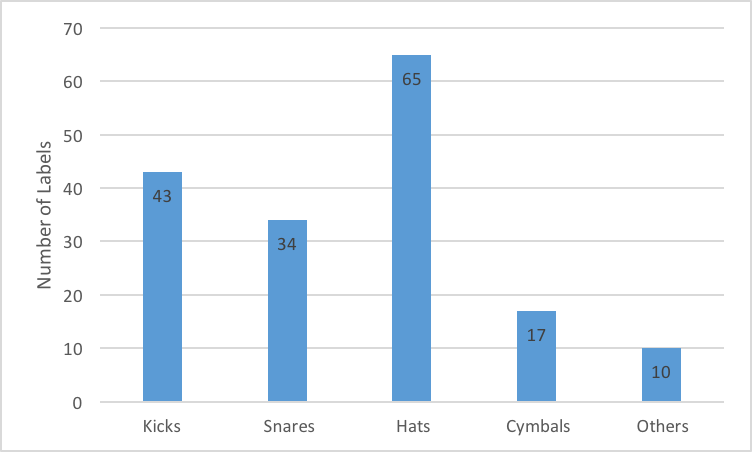
\includegraphics[width=1\linewidth]{ch07_evaluation/figures/corpus_distribution.png}
   \caption{}
   \label{fig:distrib1} 
\end{subfigure}

\begin{subfigure}[b]{0.75\textwidth}
   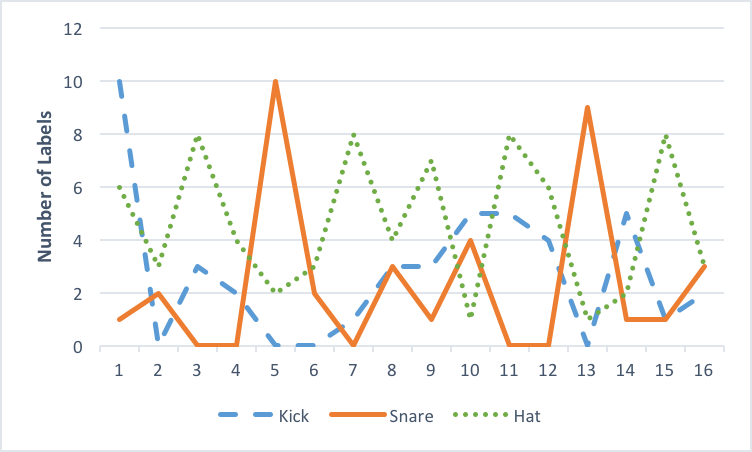
\includegraphics[width=1\linewidth]{ch07_evaluation/figures/target_distribution.png}
   \caption{}
   \label{fig:distrib2}
\end{subfigure}

\caption[Two numerical solutions]{Mean and standard deviation of fitness versus Likert scores for (a) each stimulus (b) measure and string type }
\end{figure}

\subsubsection{Retrieval Evaluation}

The aim of the experiment was first to determine how well the system was able to retrieve similarly labelled  ”units” for each 1/16th step in the seed loop. To evaluate the ability of the algorithm to retrieve correctly labelled sounds in the generated loops we defined the accuracy $A$ by \eqnref{eq:accuracy}, based on a similar approach presented by \cite{Thompson2014}.  We make a simplification that corresponding HH and X and C labels also yield a match based on our observation that their noisy qualities are very similar, and some of the target loops used did not have onsets sounding at each 1/16th step.

\begin{equation}
\label{eq:accuracy}	
A = \frac{number\;of\;correctly\;retrieved\;labels}{total\;number\;of\;labels\;in\;target}
\end{equation}  

\paragraph{Retrieval Results}

By studying the Pearson's correlation between the retrieval ratings and the distance, we can confirm the tendency of smaller distances to produce more similar patterns by observing the moderate negative correlation ($\rho = -0.516, p = 0.001$) between increased distance and the accuracy ratings (\figref{fig:corr1}).

\begin{figure}
\centering
\begin{subfigure}[b]{0.75\textwidth}
   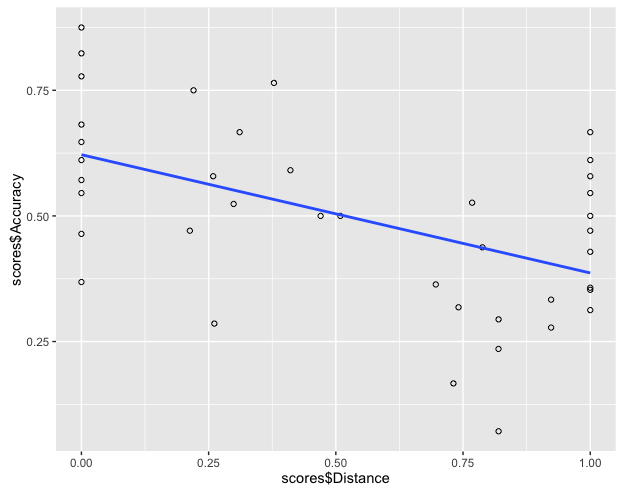
\includegraphics[width=1\linewidth]{ch07_evaluation/figures/overall_correlation.png}
   \caption{}
   \label{fig:corr1} 
\end{subfigure}

\begin{subfigure}[b]{0.75\textwidth}
   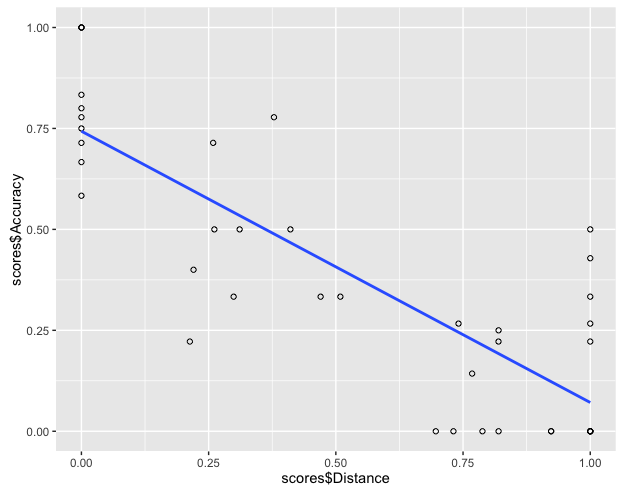
\includegraphics[width=1\linewidth]{ch07_evaluation/figures/kick_snare_correlation.png}
   \caption{}
   \label{fig:corr2}
\end{subfigure}

\caption[Two numerical solutions]{Scatterplot and Regression Line of Retrieval Accuracy for Distance for (a) all Drum Sounds (b) kick and snare isolated}
\end{figure}

An interesting observation is that when we isolate the retrieval accuracy ratings to kick and snare we see this correlation increase sharply to ($\rho = -0.826, p = 0.001$), as can be seen in \figref{fig:corr2}.

Delving into the data further, we can identify 3 different categorical groupings that demonstrate predictable trends in terms of the central tendencies and descending retrieval accuracy (\figref{fig:central_tendencies}). We label these categories A, B and C with the breakdown of the number of patterns and their corresponding distance ranges as follows:

\begin{itemize}
  \item \textit{A} - 10 Patterns - 0.0
  \item \textit{B} - 9 Patterns - [0.2 - 0.5]
  \item \textit{C} - 21 Patterns - [0.5 - 1.0]
\end{itemize}

\begin{figure}
	\begin{center}
		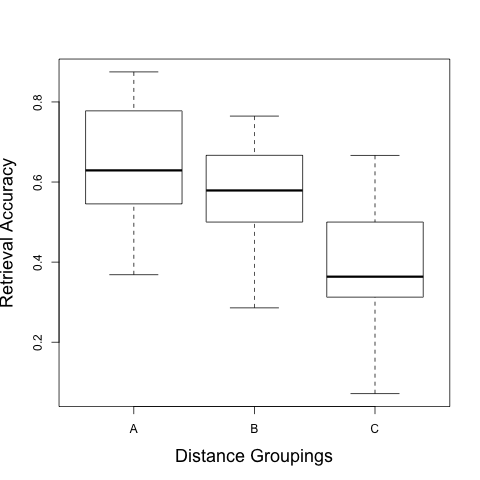
\includegraphics[width=0.6\textwidth]{ch07_evaluation/figures/new_retrieval_plot.png}
	\end{center}
	\caption[Central Tendencies of Retrieval Ratings for the Similarity/Distance Categories
]{Central Tendencies of Retrieval Ratings for the Similarity/Distance Categories}
	\label{fig:central_tendencies}
\end{figure}

\paragraph{Listener Evaluation}

The retrieval accuracy gives the objective ratings of the system’s capability for retrieving correctly labelled items. This information may not be consistent with the human listener’s perceptual impression of similarity, nor does it give any indication whether the retrieved items are musically acceptable or pleasing. To assess the human experience of the sonic output and to compare with the objective ratings of the system, we conducted a listening survey which will be described here.

To directly compare and contrast with the retrieval evaluation the same 40 loops generated by the system and used in the retrieval analysis were transferred to the listening survey. The survey itself was web-based using a modified version of the listening survey tool\footnote{SeeAppendix \ref{app:listening_survey}} used in \chapref{chap:symbolic} and took roughly 15-20 minutes to complete.

Participants were presented with the seed pattern and the generated patterns and could listen as many times as they liked. Using a 5 point Likert scale the participants were then asked to rate their agreement with the following statements:

\begin{itemize}
  \item Is the rhythmic pattern similar?
  \item Is the timbre similar?
  \item Do you like the loop?
\end{itemize}

Twenty one participants took part in total, drawn from researchers at the authors' institute of \acrshort{upf} as well as friends and colleagues with an interest in music. Twenty out of the 21 participants declared they were able to play a musical instrument.  Ten of the 21 participants specified they played a percussion instrument and 9 reported they could read notation. In the instructions we provided brief explanations of the key terms and audio examples demonstrating contrasting rhythmic patterns and timbres.

\paragraph{Listener Evaluation Results}

The survey data was analysed using Spearman's rank correlation on the mode of the participants' responses to each loop stimulus with the associated distance of that loop. We identified a moderate to strong negative correlation of -0.66, -0.59, -0.63 respectively for each of the pattern, timbre and "likeness" aspects (p < 0.01 in all instances). This can be observed in the red values in the correlation matrix presented in \figref{fig:correlation_matrix}.

\begin{figure}
	\begin{center}
		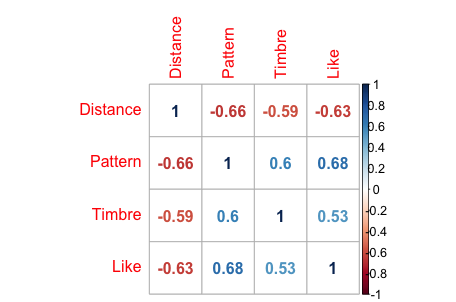
\includegraphics[width=0.75\textwidth]{ch07_evaluation/figures/correlation_matrix.png}
	\end{center}
	\caption[Correlations Between Distance and Subjective Ratings of Pattern Similarity, Timbre Similarity and Liking]{Correlations Between Distance and Subjective Ratings of Pattern Similarity, Timbre Similarity and Liking}
	\label{fig:correlation_matrix}
\end{figure}

It should be evident that the subjective listening data conforms quite well to the findings of the objective retrieval rating. Increased distance resulted in decreased retrieval accuracy which in turn corresponded to a decrease in listener ratings for qualities pertaining to pattern similarity and impression of timbral similarity in the sounds themselves. Furthermore, it was revealed that the aesthetical judgement of the generated loops, encapsulated by the "likeness" factor, also followed the trend set out by the objective algorithm. We were curious to establish whether any particular subject did not conform to this preference for similar loops, but examining the individual correlation coefficients revealed all to be negative (all participants preferred more similar sounding patterns).

\section{User Experience Evaluation}

In February 2016 we conducted several days of intensive interactive user discussions with a prototype of our system. The interviews took place at Universitat Pompeu Fabra in Barcelona and at Native Instruments Headquarters in Berlin. These interviews complement the more stringent evaluation of the system in terms of perceptual output and retrieval performance  we just saw in the previous section and published in \citep{Nuanain2016b}. This evaluation found that the retrieval ability to of the system returned greater instances of correctly labelled polyphonic drum sounds with sequences that were more similar to the target using the metric and algorithm previously described. An accompanying listener evaluation revealed that participants’ ratings correlated with our metrics in terms of similarity of pattern and timbre to the target. Additionally, the listener ratings found a correlation between closer patterns and subjective preference.

The profiles of the users for the qualitative evaluation could be divided into roughly four categories. In Barcelona, they were mostly researchers on one side, and students with a background in Sound and Music Computing on the other side. Nearly all of these participants worked with digital music in some form or other. In Berlin the users were drawn from \acrfull{rbma}\footnote{\url{http://www.redbullmusicacademy.com}} associated artists based in the city, as well as employees of Native Instruments. The \acrshort{rbma} was initiated in 1998 with the aim of gathering young music producers and DJs at worldwide events for the purposes of lectures, workshops and performances. \acrshort{rbma} collaborated in the GiantSteps project \citep{Knees2015} to provide access to these upcoming artists for research interaction and evaluation. These Berlin participants included producers, promoters, DJs, musicologists, product designers, engineers and graphic designers. United by the influence of the city, nearly everyone identified themselves as producers of techno and/or house, whether it be full-time or as a hobby.

With each participant we explained briefly the instrument and guided them through the process of generating sounds with the instrument. Mostly, the participants were eager to start playing with the instrument as soon as possible, which we were more than happy to oblige. Test stations were set up throughout the venue with a laptop, monitor and headphones as shown in \figref{fig:berlin}.

\begin{figure}
	\begin{center}
		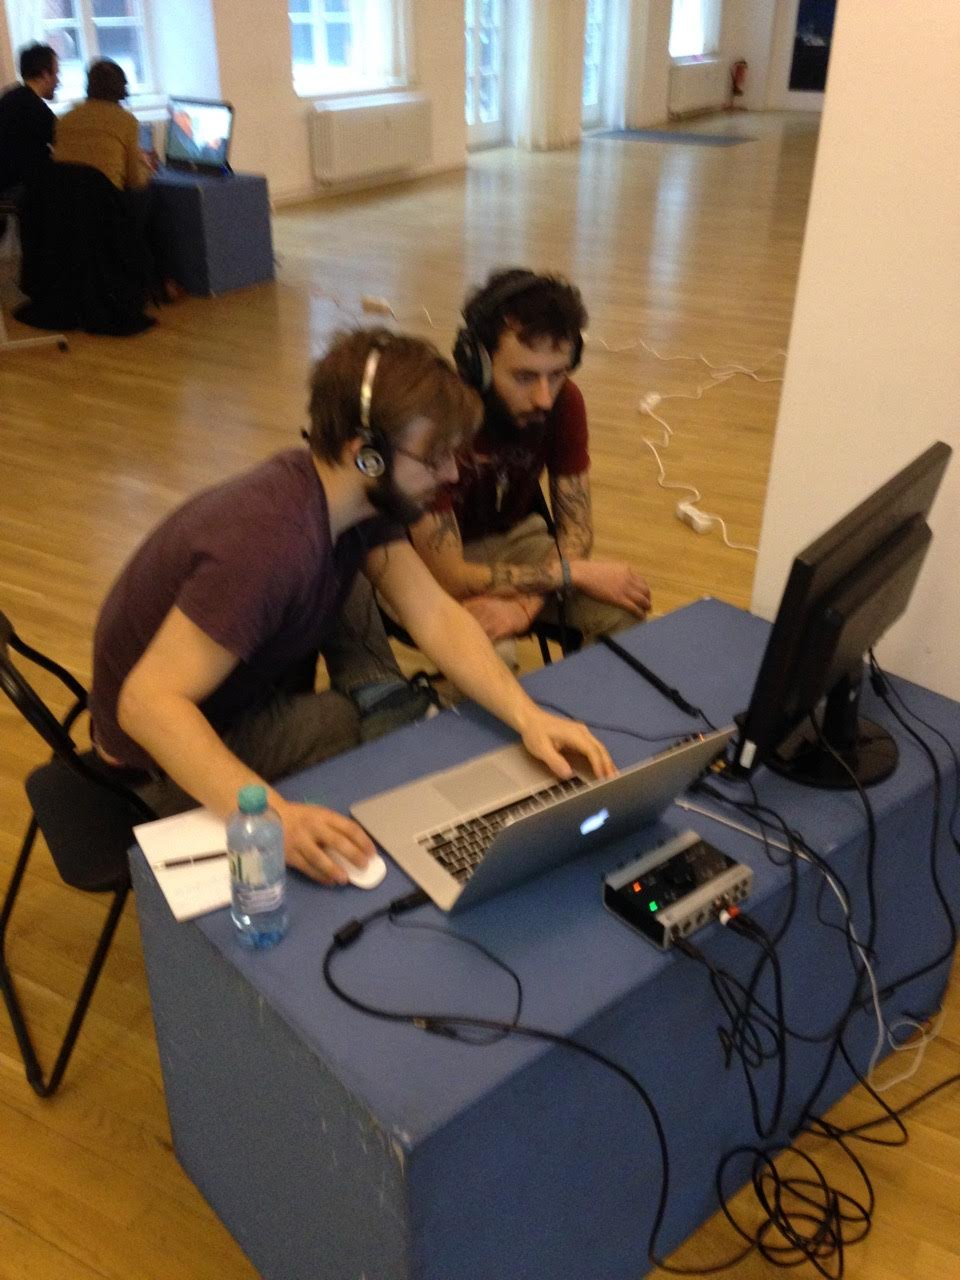
\includegraphics[width=0.4\textwidth]{ch07_evaluation/figures/berlin.jpg}
	\end{center}
	\caption[Testing Station Setup at Red Bull Music Academy in Berlin]{Testing Station Setup in at \acrshort{rbma} in Berlin}
	\label{fig:berlin}
\end{figure}

While the interviews themselves were kept informal we at least tried to steer the individual sessions with some common questions or themes in order to elicit conversation. These included statements such as:

\begin{itemize}
  \item Did the overall concept make sense to you?
  \item Was the interface intuitive? What elements were confusing?
  \item Would you use this system to make music?
  \item Would you use this system in production scenarios, live performance or both?
  \item What did you like, what didn’t you like?
  \item What improvements would you make?
  \item What features would you like to see?
\end{itemize}

\subsubsection{Positive Reactions and Outcomes}

Before delving into the specifics, we will first highlight the overall extremely positive feedback received from the participants. The word cloud in \figref{fig:wordcloud} shows a culmination of some of the frequent positive descriptions participants attached to the system during the course of the tests.

\begin{figure}
	\begin{center}
		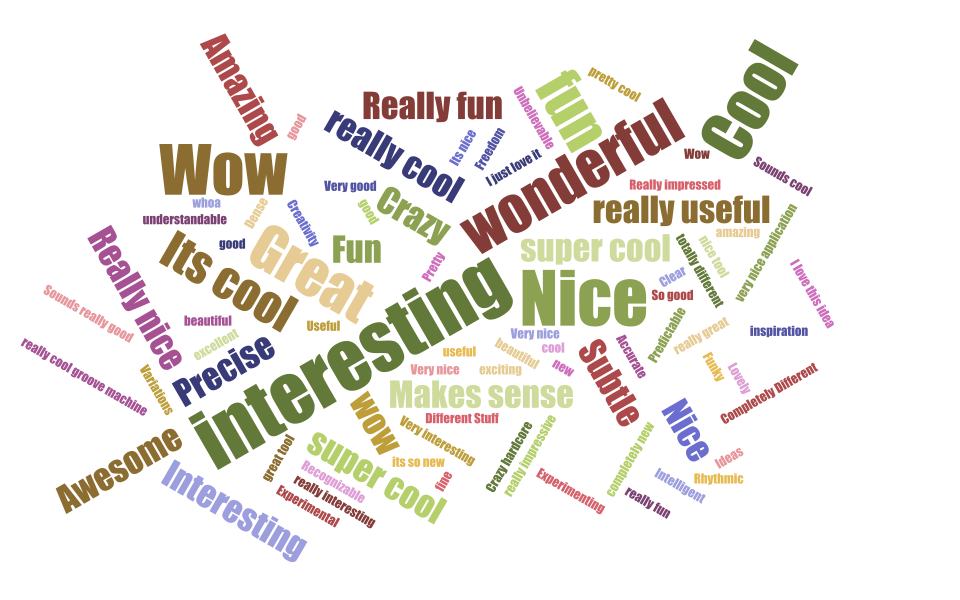
\includegraphics[width=0.85\textwidth]{ch07_evaluation/figures/wordcloud.png}
	\end{center}
	\caption[Wordcloud of most frequent positive descriptions]{Wordcloud of most frequent positive descriptions}
	\label{fig:wordcloud}
\end{figure}

Some of the more detailed positive remarks give further insights into exactly why the system appealed to them:

\blockquote{\textit{“It's an excellent tool for making small changes in real time. The interface for me is excellent. This two dimensional arrangement of the different sounds and its situation by familiarity, it's also really good for making these changes.”}}

\blockquote{\textit{“I'm really interested in more visual, more graphic interface. Also the fact that you can come up with new patterns just by the push of a button is always great.”}}

\blockquote{\textit{“It's inspiring because this mix makes something interesting still, but also I have the feeling I can steal it.”}}

\blockquote{\textit{“The unbelievable thing is that it can create something which is so accurate. I wouldn't believe that it's capable of doing such a thing.”}}

Many of the producers we spoke to reflected a particular trend in dance music at the moment for working with hardware and modular systems. This is often borne out of a desire to break out of the typical computer or digital audio workstation workflow and seek another path for inspiration.

\blockquote{\textit{“I just jam for quite a while and then try to build something that I like and then bring it to computer and then add stuff from computer. You have to jam out really. The biggest issues come with recording.”}}

The most encouraging outcome from our studies conducted with these users was that the “interesting” and “different” design of our system offers these discouraged users a way “back in” for composing with the computer once again. This was suggested by comments such as:

\blockquote{\textit{“I think something I've been looking to do in terms of experimentation and generating ideas melodically, is looking to go a bit more modular, use some modular stuff. To me, this is a digital form of it.”}}

\blockquote{\textit{“Yeah. I use a lot of hardware, but if I'd use ... a few disco breaks or something or funk breaks that would be kind of nice, totally.”}}

\subsubsection{Thematic Analysis}

We will now touch upon some of the common recurring themes that arose during the course of the interviews, and describe our own interpretations and plans to address them in future.

\paragraph{Usage Scenarios}

With respect to specific use cases, users provided some interesting scenarios where they could see the tool being used in their own interest. Numerous users were curious as to the ability to record and analyse live input such as instrumental performance or beatboxing for example.

\blockquote{\textit{“This is great! Ah, but wait. Does it mean I could like beat box really badly some idea that I have... and then bring my samples, my favourite kits and then it will just work?”}}

Live performance input was not something we had previously considered but is theoretically possible since the host would handle the capture of input audio. It would however require continuous re-analysis and computation of the similarity matrices which could be computationally costly. Still, other users have also expressed a desire for the possibility to continuously analyse incoming audio so it will be investigated.

Quite a number of users weren't interested in using the targeting capability of the synthesis engine whatsoever, and wondered if it was possible to start building patterns from scratch by selecting the onsets manually one by one. For example, referring to the fact that the dry signal is the original and the wet signal is the concatenated output:

\blockquote{\textit{ “I've got this fully on wet straight away, which tells you the direction I'd be going with it.”}}

\blockquote{\textit{“...you just want to drag in 100 different songs and you just want to explore without having this connection to the original group. Just want to explore and create sound with it.”}}

This is entirely possible; in fact, we had another "exploration" mode previously that gave the option to scan and audition the timbre space with a circular mouse radar that triggered the enclosed sounds, CataRT style. The motivation for this was to allow users to explore and audition the timbre space freely to identify regions of interest before proceeding to build their patterns. Merging this auditioning ability to create a sequence of patterns from zero would  also stem the frustration of many of the users who wanted to create sounds straight away without capturing target input.

\paragraph{Traditional Navigation}

A very early outcome of the user testing was the realisation that although users were more than open to this new way of dealing with their sound, they still wanted a link to the familiar - the  2D waveform/timeline paradigm they are so used to dealing with in existing tools such as \acrshort{daw}s.

\blockquote{\textit{“It's a bit hard to figure out which sixteenth you are looking for, because you are so used to seeing this as a step grid.”}}

\blockquote{\textit{“It's kind of good to see a different interface and not always follow the same timeline,..., But it could just be mirrored in a timeline”}}

\blockquote{\textit{“You have a waveform or something...  Then I know, okay, this is the position that I'm at.”}}

\blockquote{\textit{“Is there also a  waveform place to put the visualisation? People are so used to having that kind of thing.”}}

Initially this timeline was not something we had intended on offering; after all isn't it these paradigms we're seeking to break away from? After hearing these comments we realised that it was a useful option for the user and was one of the first items we implemented subsequently, as can be seen from \figref{fig:rhythmcat_interface}.

\paragraph{Shaping the Sounds}

Other than generating the sequences and rearranging individual units in the sequence, the synthesiser offers no additional ways to modify the output sound (discounting the ability to mix between the target sequence and the generated sequence). Many users agreed it would be useful to be able to manipulate these individual sounds sonically somehow. Most crucially they desired the option to be able to control the envelopes of the individual units via drawable Attack and Decay parameters.
  
\blockquote{\textit{“... an attack and decay just to sort of tighten it up a little bit. Get rid of some of the rough edges of the onsets and offsets.”}}

\blockquote{\textit{“Yeah, the thing is if you listen to it now, there's kind of a rhythm going, but it would be great if you could increase the decay of the snare for example. Which if it's prototype, you can't expect to have all those functions there immediately, but in an end product, I think it would be a necessity.”}}

\paragraph{State and Feedback}

One of the consistent items that concern users of generative systems is the notion of state. On a superficial level state can refer to an effective preset management system that stores their efforts, for as one participant notes "you're always afraid of losing something.". Users are terrified of losing their progress once they've entered a pleasing "state", although this is a much bigger concern in probabilistic systems that produce - but then may never reproduce - "happy accidents".

At present our system has no state, and this was something frequently remarked upon and something we are actively considering. Users expressed a desire for complex state operations. Comparing two generated sequences visually and sonically for example, and being able to mix or find an interpolation between the two of them somehow. One artist wondered whether would it be possible to extend the graph visualisation technique to a space of "patterns". In this manner a series of stored patterns would be plotted in 2D space one after each other, and could be explored and sequenced in a more high-level arrangement or score-type interaction with the instrument. As he explained:

\blockquote{\textit{“Even with this if it wasn't actually blending or interpolating between points, but just so you could save the state in a composition screen of dots and you could just jump between.”}}

This was actually inspired by the artist's own experiences with another experimental but commercial tool for music production: Audiomulch[33]. It includes a unique feature known as the MetaSurface, which allows navigation and interpolation of multiple parameter states by manipulating a colourful visual cluster space.

Also related to issue of state was the ability to initiate feedback, i.e. continuously assigning the concatenated output to the input, which once again can be done manually by recording to the host and re-recording in. This could be facilitated in the tool itself, but would require having the option of removing the matching sounds from the corpus itself to encourage diversity of sound.

\paragraph{Parameterisation and Visualisation}

One of the recurring difficulties that faced participants was our presentation of the parameters. As we explained briefly in the implementation section, the user is able to control the influence of the four features in concatenation algorithm and the PCA visualisation. We relabelled the features from their objective names to what we considered a subjective equivalent that a lay user may understand. MFCCs are labelled as "Timbre", spectral centroid as "Brightness", spectral flatness as "harmonicity" with Loudness unchanged.  

Unfortunately, users expressed confusion at their purpose and were unable to interpret their effect on neither the arrangement of the units of sound in space or their resulting effect on the patterns generated. For instance:

\blockquote{\textit{
“The problem is I'm a little bit lost already.”\\\\
“you have four parameters, and you don't know which thing is what”\\\\
“I would prefer not to have too much controls.”
}}

Presenting this additional complexity was a perhaps naive inclusion on our part. Clearly the typical user is content with the overall output from the system and would rather not delve into these specifics. However, at least in terms of the visualisation there is a "sweet spot" for feature weightings in the arrangement of the units of sound in the timbre space and this is why the controls were made available. The weightings can vary greatly depending on the corpus, though in our experience \acrshort{mfcc} alone often provide the best separation and clustering.

The challenge will be to find the best approach to arranging the units in sound with the best separation and shielding these parameters from the user. Potentially, a way forward could be to remove these sliders and replace them with a number of options including an “advanced” mode with the ability to select specific parameters for the axes like CataRT in addition to “automatic” arrangement presets made possible using dimensionality reduction techniques. An area for study would be to gather many different sound sets and try various combinations of feature selections and weightings to find the best visual separation. At present \acrshort{pca} is used for dimension reduction but as we reported in \chapref{chap:rhythmcat} there also exists \acrshort{mds} and \acrshort{tsne} which we have yet to offer to the user. In our informal experiments with the latter we have noticed two immediate drawbacks in its applicability for real-time or at least `production ready' usage. Firstly, a successful projection, encompassing good separation with minimal overlapping of clusters, is heavily dependent on tweaking the parameters of the system to the data provided. Secondly, the algorithm is complex enough that it needs to pass through a number of iterations before it finally settles on a projection with minimal threshold error, thus there is a delay in the time it takes for it to project (however we have observed that this makes a rather nice dynamic animation when its processing routine is placed in the interface update loop!). 
